\let\negmedspace\undefined
\let\negthickspace\undefined
\documentclass[journal,12pt,onecolumn]{IEEEtran}
\usepackage{cite}
\usepackage{amsmath,amssymb,amsfonts,amsthm}
\usepackage{algorithmic}
\usepackage{graphicx}
\usepackage{textcomp}
\usepackage{xcolor}
\usepackage{txfonts}
\usepackage{listings}
\usepackage{enumitem}
\usepackage{mathtools}
\usepackage{gensymb}
\usepackage[breaklinks=true]{hyperref}
\usepackage{tkz-euclide} % loads  TikZ and tkz-base
\usepackage{listings}



\newtheorem{theorem}{Theorem}[section]
\newtheorem{problem}{Problem}
\newtheorem{proposition}{Proposition}[section]
\newtheorem{lemma}{Lemma}[section]
\newtheorem{corollary}[theorem]{Corollary}
\newtheorem{example}{Example}[section]
\newtheorem{definition}[problem]{Definition}
%\newtheorem{thm}{Theorem}[section] 
%\newtheorem{defn}[thm]{Definition}
%\newtheorem{algorithm}{Algorithm}[section]
%\newtheorem{cor}{Corollary}
\newcommand{\BEQA}{\begin{eqnarray}}
\newcommand{\EEQA}{\end{eqnarray}}
\newcommand{\define}{\stackrel{\triangle}{=}}
\theoremstyle{remark}
\newtheorem{rem}{Remark}
%\bibliographystyle{ieeetr}
\begin{document}
%
\providecommand{\pr}[1]{\ensuremath{\Pr\left(#1\right)}}
\providecommand{\prt}[2]{\ensuremath{p_{#1}^{\left(#2\right)} }}        % own macro for this question
\providecommand{\qfunc}[1]{\ensuremath{Q\left(#1\right)}}
\providecommand{\sbrak}[1]{\ensuremath{{}\left[#1\right]}}
\providecommand{\lsbrak}[1]{\ensuremath{{}\left[#1\right.}}
\providecommand{\rsbrak}[1]{\ensuremath{{}\left.#1\right]}}
\providecommand{\brak}[1]{\ensuremath{\left(#1\right)}}
\providecommand{\lbrak}[1]{\ensuremath{\left(#1\right.}}
\providecommand{\rbrak}[1]{\ensuremath{\left.#1\right)}}
\providecommand{\cbrak}[1]{\ensuremath{\left\{#1\right\}}}
\providecommand{\lcbrak}[1]{\ensuremath{\left\{#1\right.}}
\providecommand{\rcbrak}[1]{\ensuremath{\left.#1\right\}}}
\newcommand{\sgn}{\mathop{\mathrm{sgn}}}
\providecommand{\abs}[1]{\left\vert#1\right\vert}
\providecommand{\res}[1]{\Res\displaylimits_{#1}} 
\providecommand{\norm}[1]{\left\lVert#1\right\rVert}
%\providecommand{\norm}[1]{\lVert#1\rVert}
\providecommand{\mtx}[1]{\mathbf{#1}}
\providecommand{\mean}[1]{E\left[ #1 \right]}
\providecommand{\cond}[2]{#1\middle|#2}
\providecommand{\fourier}{\overset{\mathcal{F}}{ \rightleftharpoons}}
\newenvironment{amatrix}[1]{%
  \left(\begin{array}{@{}*{#1}{c}|c@{}}
}{%
  \end{array}\right)
}
%\providecommand{\hilbert}{\overset{\mathcal{H}}{ \rightleftharpoons}}
%\providecommand{\system}{\overset{\mathcal{H}}{ \longleftrightarrow}}
	%\newcommand{\solution}[2]{\textbf{Solution:}{#1}}
\newcommand{\solution}{\noindent \textbf{Solution: }}
\newcommand{\cosec}{\,\text{cosec}\,}
\providecommand{\dec}[2]{\ensuremath{\overset{#1}{\underset{#2}{\gtrless}}}}
\newcommand{\myvec}[1]{\ensuremath{\begin{pmatrix}#1\end{pmatrix}}}
\newcommand{\mydet}[1]{\ensuremath{\begin{vmatrix}#1\end{vmatrix}}}
\newcommand{\myaugvec}[2]{\ensuremath{\begin{amatrix}{#1}#2\end{amatrix}}}
\providecommand{\rank}{\text{rank}}
\providecommand{\pr}[1]{\ensuremath{\Pr\left(#1\right)}}
\providecommand{\qfunc}[1]{\ensuremath{Q\left(#1\right)}}
	\newcommand*{\permcomb}[4][0mu]{{{}^{#3}\mkern#1#2_{#4}}}
\newcommand*{\perm}[1][-3mu]{\permcomb[#1]{P}}
\newcommand*{\comb}[1][-1mu]{\permcomb[#1]{C}}
\providecommand{\qfunc}[1]{\ensuremath{Q\left(#1\right)}}
\providecommand{\gauss}[2]{\mathcal{N}\ensuremath{\left(#1,#2\right)}}
\providecommand{\diff}[2]{\ensuremath{\frac{d{#1}}{d{#2}}}}
\providecommand{\myceil}[1]{\left \lceil #1 \right \rceil }
\newcommand\figref{Fig.~\ref}
\newcommand\tabref{Table~\ref}
\newcommand{\sinc}{\,\text{sinc}\,}
\newcommand{\rect}{\,\text{rect}\,}
%%
%	%\newcommand{\solution}[2]{\textbf{Solution:}{#1}}
%\newcommand{\solution}{\noindent \textbf{Solution: }}
%\newcommand{\cosec}{\,\text{cosec}\,}
%\numberwithin{equation}{section}
%\numberwithin{equation}{subsection}
%\numberwithin{problem}{section}
%\numberwithin{definition}{section}
%\makeatletter
%\@addtoreset{figure}{problem}
%\makeatother

%\let\StandardTheFigure\thefigure
\let\vec\mathbf


\bibliographystyle{IEEEtran}
\title{ GATE CH-23 44}
\author{EE23BTECH11011- Batchu Ishitha$^{*}$% <-this % stops a space
}
\maketitle




\bigskip

\renewcommand{\thefigure}{\theenumi}
\renewcommand{\thetable}{\theenumi}
%\renewcommand{\theequation}{\theenumi}

Q: A cascade control strategy is shown in the figure below. The transfer function between the output $(y)$ and the secondary disturbance $(d_2)$ is defined as  \\
$$G_{d2}(s)= \frac{y(s)}{d_2(s)}$$. 
Which one of the following is the CORRECT expression for the transfer function $G_{d2}(s)$? \\
\begin{figure}[h]
    \centering
    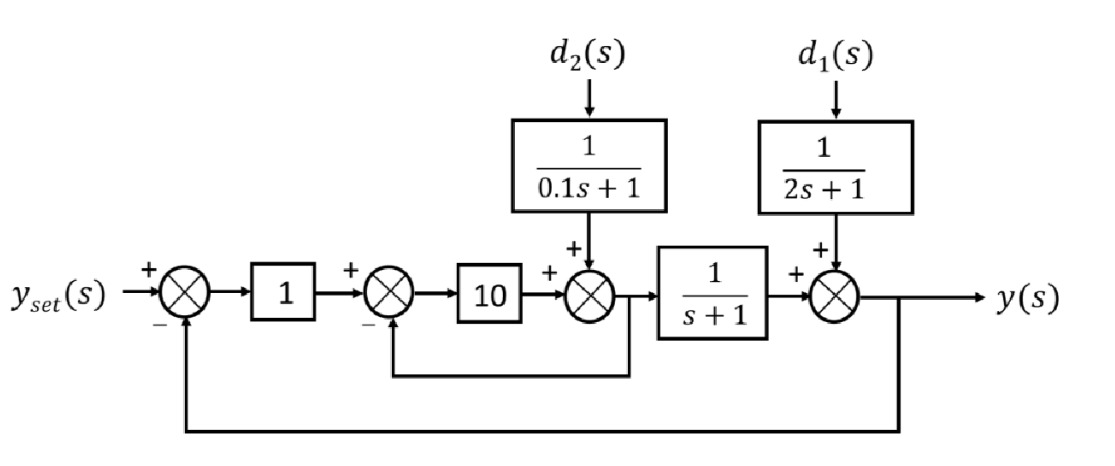
\includegraphics[width=\columnwidth]{../gate23.ch.44/figs/g44fig1.jpeg}
    \caption{ }
    \label{}
\end{figure}
\begin{enumerate}[label=\Alph*.]
\item $\frac{1}{(11s+21)(0.1s+1)}$ 
\item $\frac{1}{(s+1)(0.1s+1)}$
\item $\frac{(s+1)}{(s+2)(0.1s+1)}$
\item $\frac{(s+1)}{(s+1)(0.1s+1)}$
\end{enumerate}

\solution 

\begin{table}[!ht]
    \centering
              \begin{tabular}{|c|c|} 
      \hline
\textbf{Variable}& \textbf{Description}\\\hline
         $d_1(s)$& Primary disturbance \\\hline
         $d_2(s)$& Secondary disturbance \\\hline
         $G_{d2}(s)$&Transfer function between $y(s)$ and $d_2(s)$\\\hline
         $y_{set}(s)$& Set point for desired output \\\hline
         $y(s)$ & Output \\\hline
        \end{tabular}
        
        

    \caption{Input Parameters}
    \label{tab: ishithagatech44.t1}
\end{table}

\begin{table}[!ht]
    \centering
            \begin{tabular}{|c|c|c|} 
    \hline
\textbf{Variable}& \textbf{Description} & \textbf{value}\\\hline
    $P_{1}$& Forward path gain e-c-d & $\frac{1}{\brak{0.1s+1}\brak{s+1}}$\\\hline
    $\Delta_{1}$&Determinant of forward path e-c-d & $1$\\\hline
    $\Delta$& Determinant of system & $1+\frac{10}{s+1}+10$\\\hline
    $n$& Number of forward path & $1$\\\hline
    \end{tabular}

    \caption{Defined Parameters}
    \label{tab: ishithagatech44.t2}
\end{table}

\begin{figure}[!ht]
    \centering
    \usetikzlibrary{decorations.markings}
\newif\iflabrev

\begin{tikzpicture}
[
label revd/.is if=labrev,
%label revd/.default=true,
amark/.style={
            decoration={             
                        markings,   
                        mark=at position {0.5} with { 
                                    \arrow{stealth},
                                    \iflabrev \node[above] {#1};\else \node[below] {#1};\fi
                        }
            },
            postaction={decorate}
},
terminal/.style 2 args={draw,circle,inner sep=2pt,label={#1:#2}},
]

%Place the nodes
\node[terminal={below}{$Y_{set}(s)$}] (ysp) at (0,0) {};
\node[terminal={above left}{$a$}] (a) at (1.5,0) {};
\node[terminal={above left}{$b$}] (b) at (3,0) {};
\node[terminal={above right}{$c$}] (c) at (4.5,0) {};
\node[terminal={above right}{$d$}] (d) at (6,0) {};
\node[terminal={right}{$e$}] (e) at (4.5,-1.5) {};
\node[terminal={left}{$f$}] (f) at (6,-1.5) {};
\node[terminal={below}{$Y(s)$}] (ys) at (7.5,0) {};
\node[terminal={left}{$d_2(s)$}] (d2s) at (4.5,-3) {};
\node[terminal={left}{$d_1(s)$}] (d1s) at (6,-3) {};

%Draw the connections
\draw[amark](ysp) to (a);
\draw[amark=$1$] (a) to (b);
\draw[amark=$10$] (b) to (c);
\draw[amark=$-1$,label revd] (b) to[bend left=90] (c);
\draw[amark=$\frac{1}{s+1}$] (c) to (d);
\draw[amark] (d) to (ys);
\draw[amark=$-1$,label revd] (a) to[bend left=90] (d);
\draw[amark] (e) to node[midway, below left] {$\frac{1}{0.1s+1}$} (c);
\draw[amark] (f) to node[midway, below right] {$\frac{1}{2s+1}$} (d);
\draw[amark](d2s) to (e);
\draw[amark](d1s) to (f);
\end{tikzpicture}

    \caption{signal flow graph}
    \label{fig:ishitha.g23.ch.44.f1}
\end{figure}

\newpage
Using Mason's Gain formula for the above Signal flow graph,

\begin{align}
G_{d2}(s) = \frac{y(s)}{d_2(s)} &= \frac{{\sum_{i=1}^{n} P_i\Delta_i}}{{\Delta}} \\
&= \frac{P_1\Delta_1 }{\Delta}\\
&= \frac{\frac{1}{\brak{0.1s+1}\brak{s+1}}}{1+\frac{10}{s+1}+10} \\
&= \frac{\frac{1}{\brak{0.1s+1}\brak{s+1}}}{\frac{11s+21}{s+1}} \\
\implies G_{d2}(s) &= \frac{1}{(11s+21)(0.1s+1)}
\end{align}

Now taking the inverse laplace transform we have,
\begin{align}
G_{d2}(t) &= \mathcal{L}^{-1}\brak{\frac{10}{\brak{s+10}\brak{11s+21}}} \\
&=\mathcal{L}^{-1}{\brak{\frac{-10}{89\brak{x+10}} + \frac{110}{89\brak{11x+21}}}} \\
&= \frac{-10e^{-10t}}{89} + \frac{10e^{\frac{-21t}{11}}}{89} \\
&= \frac{10\brak{e^{\frac{-21t}{11}}-e^{-10t}}}{89}
\end{align}

\begin{figure}[!ht]
    \centering
     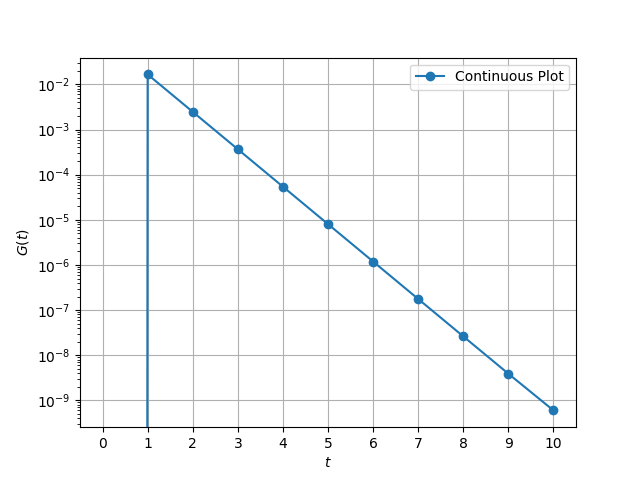
\includegraphics[width=\columnwidth]{./figs/g44fig1.png}
    \caption{}    
    \label{fig:ishitha.g23.ch.44.f2}
\end{figure}

\end{document}
